\documentclass[11pt,a4paper]{article}

\usepackage[margin=1in]{geometry}
\usepackage{amsmath,amssymb,amsthm}
\usepackage{booktabs}
\usepackage{graphicx}
\usepackage{caption}
\usepackage{subcaption}
\usepackage{listings}
\usepackage{xcolor}
\usepackage[round]{natbib}
\usepackage{hyperref}

\hypersetup{colorlinks=true, urlcolor=blue, linkcolor=black, citecolor=blue}

\lstset{
  basicstyle=\ttfamily\footnotesize,
  breaklines=true,
  showstringspaces=false,
  frame=single,
  rulecolor=\color{black!30}
}

\title{Research Assistant Test for ERC Really Credible }
\author{Siddhant Manav Pagare }
\date{May 2026}

\begin{document}

\maketitle

\newpage

\section*{Exercise 1}
% Exercise 1, super consistent estimator.


\noindent \textbf{Given.} $(Y_i)_{1 \le i \le n}$ iid with $Y_i \sim \mathcal{U}[0, \theta]$ for an unknown $\theta > 0$. \\

We are asked to compare two estimators of $\theta$, the method of moments estimator $\widehat\theta_{MM} = 2 \bar Y_n$ and the maximum likelihood estimator $\widehat\theta_{ML} = \max_i Y_i$, and use the better of the two to build a confidence interval for $\theta$.

\subsection*{Part (a)}

We are given that $Y \sim \mathcal{U}[0, \theta]$ with density $f(y) = 1/\theta$ on $[0, \theta]$. We compute the expectation by direct integration:
\[
E(Y) = \int_0^\theta y \cdot \frac{1}{\theta}\, dy = \frac{\theta}{2}.
\]
Rearranging, $\theta = 2 E(Y)$. The unknown $\theta$ is exactly twice the population mean of $Y$. This identity is the bridge we use in the next part to build an estimator: any sensible estimator of $E(Y)$ doubles to an estimator of $\theta$.

\subsection*{Part (b)}

The method of moments substitutes population expectations by their sample analogues. We replace $E(Y)$ in the identity $\theta = 2 E(Y)$ from part (a) by the sample mean $\bar Y_n = n^{-1} \sum_{i=1}^n Y_i$, which gives
\[
\widehat\theta_{MM} = 2 \bar Y_n.
\]
Because $\widehat\theta_{MM} = 2 \bar Y_n$ is an affine function of $\bar Y_n$, its sampling moments follow directly from those of $\bar Y_n$ by the standard rules for affine transformations of a random variable. For the mean,
\[
E(\widehat\theta_{MM}) = E(2 \bar Y_n) = 2 E(\bar Y_n).
\]
For the variance, applying the rule $\mathrm{Var}(a X) = a^2 \mathrm{Var}(X)$ with $a = 2$,
\[
\mathrm{Var}(\widehat\theta_{MM}) = \mathrm{Var}(2 \bar Y_n) = 2^2 \mathrm{Var}(\bar Y_n) = 4 \mathrm{Var}(\bar Y_n).
\]
We will use both of these in part (c) and part (g).

\subsection*{Part (c)}

We show $\widehat\theta_{MM}$ is asymptotically normal with asymptotic variance $4 V(Y)$. The only assumption needed is finite variance of $Y$, which is automatic since $Y$ takes values in the bounded interval $[0, \theta]$, so all moments exist.

The central limit theorem applies to the sample mean of iid variables with finite variance, and gives
\[
\sqrt{n}\bigl(\bar Y_n - E(Y)\bigr) \overset{d}{\longrightarrow} \mathcal{N}\bigl(0, V(Y)\bigr).
\]
We need to turn this into a statement about $\widehat\theta_{MM}$. Start from two identities derived earlier:
\[
\widehat\theta_{MM} = 2 \bar Y_n \quad \text{(part (b))}, \qquad \theta = 2 E(Y) \quad \text{(part (a))}.
\]
Subtracting the second from the first,
\[
\widehat\theta_{MM} - \theta = 2 \bar Y_n - 2 E(Y) = 2\bigl(\bar Y_n - E(Y)\bigr).
\]
Multiplying both sides by $\sqrt n$,
\[
\sqrt{n}\bigl(\widehat\theta_{MM} - \theta\bigr) = \sqrt{n} \cdot 2\bigl(\bar Y_n - E(Y)\bigr) = 2 \cdot \sqrt{n}\bigl(\bar Y_n - E(Y)\bigr).
\]
The right hand side is two times a sequence whose limit law we already have from the central limit theorem. We now invoke the following general fact: if $T_n \overset{d}{\longrightarrow} \mathcal{N}(0, \sigma^2)$ and $a$ is a real constant, then $a T_n \overset{d}{\longrightarrow} a \cdot \mathcal{N}(0, \sigma^2)$. Furthermore, multiplying a centred normal by a constant $a$ rescales its variance by $a^2$, that is $a \cdot \mathcal{N}(0, \sigma^2) = \mathcal{N}(0, a^2 \sigma^2)$. Applying this with $a = 2$, $T_n = \sqrt n (\bar Y_n - E(Y))$, $\sigma^2 = V(Y)$,
\[
\sqrt{n}\bigl(\widehat\theta_{MM} - \theta\bigr) \overset{d}{\longrightarrow} 2 \cdot \mathcal{N}\bigl(0, V(Y)\bigr) = \mathcal{N}\bigl(0, 2^2 V(Y)\bigr) = \mathcal{N}\bigl(0, 4 V(Y)\bigr).
\]
The asymptotic variance is therefore $4 V(Y)$, as claimed.

For our specific uniform model we compute $V(Y)$ directly. The second moment is
\[
E(Y^2) = \int_0^\theta y^2 \cdot \frac{1}{\theta}\, dy = \frac{1}{\theta} \cdot \frac{\theta^3}{3} = \frac{\theta^2}{3},
\]
and combined with $E(Y) = \theta/2$ from part (a),
\[
V(Y) = E(Y^2) - E(Y)^2 = \frac{\theta^2}{3} - \left(\frac{\theta}{2}\right)^2 = \frac{\theta^2}{3} - \frac{\theta^2}{4} = \frac{4 \theta^2 - 3 \theta^2}{12} = \frac{\theta^2}{12}.
\]
The asymptotic variance therefore evaluates to $4 V(Y) = 4 \cdot \theta^2/12 = \theta^2/3$. The estimator $\widehat\theta_{MM}$ is $\sqrt n$ consistent: its error shrinks at the standard rate $1/\sqrt n$.

\subsection*{Part (d)}

The alternative estimator $\widehat\theta_{ML} = \max_{1 \le i \le n} Y_i$ is natural for two reasons that we will both use later.

First, by the support of the distribution, $Y_i \le \theta$ for every $i$, so the sample maximum is always at most $\theta$ and accumulates near $\theta$ as $n$ grows. The maximum is therefore a sensible lower bound for $\theta$ that tightens with sample size.

Second, $\widehat\theta_{ML}$ is the maximum likelihood estimator. The joint density of the sample is
\[
f(y_1, \dots, y_n; \theta) = \prod_{i=1}^n \frac{1}{\theta} \mathbf{1}\{0 \le y_i \le \theta\} = \frac{1}{\theta^n}\, \mathbf{1}\bigl\{\max_i y_i \le \theta\bigr\},
\]
which is zero on the inadmissible region $\theta < \max_i y_i$. On the admissible region $\theta \ge \max_i y_i$, the indicator equals one and the likelihood reduces to
\[
L(\theta) = \theta^{-n}.
\]
Differentiating with respect to $\theta$,
\[
\frac{d L}{d \theta} = -n\, \theta^{-(n+1)} < 0 \quad \text{for every } \theta > 0,
\]
so $L$ is strictly decreasing on the admissible region. The likelihood is therefore maximised at the smallest admissible value of $\theta$, which is the smallest $\theta$ satisfying $\theta \ge \max_i y_i$, namely
\[
\widehat\theta_{ML} = \max_i Y_i.
\]
The two views agree.

\subsection*{Part (e)}

To analyse the asymptotic behaviour of $\widehat\theta_{ML}$ in part (f) we first need its full cdf. The event $\{\max_i Y_i \le x\}$ is the same as $\{Y_1 \le x \text{ and } \dots \text{ and } Y_n \le x\}$. Independence of the $Y_i$ then turns the joint probability into a product, and the marginal cdf of the uniform gives $P(Y_i \le x) = x/\theta$ for $x \in [0, \theta]$. Putting these together,
\[
P\bigl(\widehat\theta_{ML} \le x\bigr) = \prod_{i=1}^n P(Y_i \le x) = \left(\frac{x}{\theta}\right)^n
\]
for $x \in [0, \theta]$. The event is impossible for $x < 0$ and certain for $x > \theta$, so
\[
P\bigl(\widehat\theta_{ML} \le x\bigr) =
\begin{cases}
0 & \text{if } x < 0, \\
(x/\theta)^n & \text{if } x \in [0, \theta], \\
1 & \text{if } x > \theta.
\end{cases}
\]
The cdf concentrates rapidly near $\theta$ as $n$ grows. The next part turns this into a precise rate.

\subsection*{Part (f)}

We show that $Z_n = n(\theta - \widehat\theta_{ML})/\theta$ converges in distribution to $U \sim \mathrm{Exp}(1)$. Following the hint in the problem, the strategy is to verify pointwise convergence of the cdf of $Z_n$ to the cdf of $\mathrm{Exp}(1)$ at every continuity point. The target cdf
\[
F(x) = \begin{cases} 0 & x < 0, \\ 1 - \exp(-x) & x \ge 0, \end{cases}
\]
is continuous on all of $\mathbb{R}$, so we need pointwise convergence at every $x$.

Consider $x < 0$ first. Since $\widehat\theta_{ML} \le \theta$ almost surely (the support argument from part (d)), $Z_n \ge 0$ almost surely, so $P(Z_n \le x) = 0 = F(x)$.

For $x \ge 0$, and $n$ large enough that $x/n \le 1$ so that $\theta(1 - x/n) \in [0, \theta]$, we first rewrite the event $\{Z_n \le x\}$ in terms of $\widehat\theta_{ML}$. Starting from the definition of $Z_n$ and rearranging step by step,
\begin{align*}
Z_n \le x
&\iff \frac{n(\theta - \widehat\theta_{ML})}{\theta} \le x \\
&\iff n(\theta - \widehat\theta_{ML}) \le x \theta && \text{(multiply both sides by $\theta > 0$)} \\
&\iff \theta - \widehat\theta_{ML} \le \frac{x \theta}{n} && \text{(divide both sides by $n > 0$)} \\
&\iff \widehat\theta_{ML} \ge \theta - \frac{x \theta}{n} && \text{(rearrange)} \\
&\iff \widehat\theta_{ML} \ge \theta\left(1 - \frac{x}{n}\right) && \text{(factor out $\theta$)}.
\end{align*}
Each rearrangement preserves the inequality because every multiplier is strictly positive ($\theta > 0$, $n > 0$). Taking probabilities and applying the cdf from part (e),
\begin{align*}
P(Z_n \le x)
&= P\bigl(\widehat\theta_{ML} \ge \theta(1 - x/n)\bigr) \\
&= 1 - P\bigl(\widehat\theta_{ML} < \theta(1 - x/n)\bigr) && \text{(complement)} \\
&= 1 - \left(\frac{\theta(1 - x/n)}{\theta}\right)^n && \text{(cdf from part (e))} \\
&= 1 - (1 - x/n)^n && \text{($\theta$ cancels)}.
\end{align*}
The standard analysis limit $(1 - x/n)^n \to \exp(-x)$ as $n \to \infty$ then yields
\[
P(Z_n \le x) \to 1 - \exp(-x) = F(x).
\]
Combining the two cases, $P(Z_n \le x) \to F(x)$ pointwise, so $Z_n \overset{d}{\longrightarrow} \mathrm{Exp}(1)$. \qed

This is the rate result. The error $\theta - \widehat\theta_{ML}$ shrinks at rate $1/n$ rather than the standard $1/\sqrt n$, so $\widehat\theta_{ML}$ is super consistent. Part (g) cashes this in.

\subsection*{Part (g)}

We now compare the two estimators. From part (c), $\widehat\theta_{MM}$ is $\sqrt n$ consistent with asymptotic variance $\theta^2/3$. From part (f), $\widehat\theta_{ML}$ is $n$ consistent. The contrast is therefore between rates $1/\sqrt n$ and $1/n$.

\textit{MSE for $\widehat\theta_{MM}$.} The MM estimator is unbiased:
\[
E(\widehat\theta_{MM}) = 2 E(\bar Y_n) = 2 E(Y) = 2 \cdot \frac{\theta}{2} = \theta.
\]
Combining the variance scaling from part (b) with $V(Y) = \theta^2/12$ from part (c),
\[
\mathrm{Var}(\widehat\theta_{MM}) = 4 \mathrm{Var}(\bar Y_n) = 4 \cdot \frac{V(Y)}{n} = 4 \cdot \frac{\theta^2/12}{n} = \frac{\theta^2}{3 n}.
\]
Since the bias is zero, $\mathrm{MSE}(\widehat\theta_{MM}) = \mathrm{Var}(\widehat\theta_{MM}) = \theta^2/(3 n)$.

\textit{MSE for $\widehat\theta_{ML}$.} The exact finite sample moments of $\widehat\theta_{ML}$ follow from order statistic theory. Differentiating the cdf from part (e) gives the density on $[0, \theta]$,
\[
f_{\widehat\theta_{ML}}(x) = \frac{d}{dx}\left(\frac{x}{\theta}\right)^n = \frac{n x^{n-1}}{\theta^n}.
\]
Computing the first two moments by direct integration,
\[
E(\widehat\theta_{ML}) = \int_0^\theta x \cdot \frac{n x^{n-1}}{\theta^n}\, dx = \frac{n}{\theta^n} \cdot \frac{\theta^{n+1}}{n+1} = \frac{n}{n+1}\, \theta,
\]
\[
E(\widehat\theta_{ML}^2) = \int_0^\theta x^2 \cdot \frac{n x^{n-1}}{\theta^n}\, dx = \frac{n}{\theta^n} \cdot \frac{\theta^{n+2}}{n+2} = \frac{n}{n+2}\, \theta^2,
\]
and therefore
\[
\mathrm{Var}(\widehat\theta_{ML}) = E(\widehat\theta_{ML}^2) - E(\widehat\theta_{ML})^2 = \frac{n \theta^2}{n+2} - \frac{n^2 \theta^2}{(n+1)^2} = \frac{n \theta^2}{(n+1)^2 (n+2)},
\]
after putting over a common denominator and simplifying. The bias is
\[
E(\widehat\theta_{ML}) - \theta = \frac{n \theta}{n+1} - \theta = \frac{n \theta - (n+1) \theta}{n+1} = -\frac{\theta}{n+1},
\]
so $\widehat\theta_{ML}$ is biased downward by $\theta/(n+1)$. The bias and the standard deviation both shrink at rate $1/n$, so neither dominates the other. The mean squared error decomposes as
\begin{align*}
\mathrm{MSE}(\widehat\theta_{ML})
&= \mathrm{Bias}^2 + \mathrm{Var}(\widehat\theta_{ML}) \\
&= \left(\frac{\theta}{n+1}\right)^2 + \frac{n \theta^2}{(n+1)^2 (n+2)} \\
&= \frac{\theta^2}{(n+1)^2} + \frac{n \theta^2}{(n+1)^2 (n+2)} \\
&= \frac{\theta^2}{(n+1)^2} \left[1 + \frac{n}{n+2}\right] \\
&= \frac{\theta^2}{(n+1)^2} \cdot \frac{(n+2) + n}{n+2} \\
&= \frac{\theta^2 (2 n + 2)}{(n+1)^2 (n+2)} \\
&= \frac{2 \theta^2 (n+1)}{(n+1)^2 (n+2)} \\
&= \frac{2 \theta^2}{(n+1)(n+2)}.
\end{align*}

\textit{Comparison.} The MM mean squared error $\theta^2/(3n)$ decays at rate $1/n$. The ML mean squared error $2 \theta^2 / ((n+1)(n+2))$ decays at rate $1/n^2$. At $n = 1000$ and $\theta = 1$,
\[
\mathrm{MSE}(\widehat\theta_{MM}) \approx \frac{1}{3000} \approx 3.3 \times 10^{-4}, \qquad
\mathrm{MSE}(\widehat\theta_{ML}) \approx \frac{2}{1001 \cdot 1002} \approx 2 \times 10^{-6},
\]
two orders of magnitude apart.

The ML estimator is the better estimator. The downward bias does not change the comparison because the rate gain dominates.

\subsection*{Part (h)}

We confirm the rate comparison numerically in Stata. The single sample exercise asks for $n = 1000$ draws from $\mathcal{U}[0, 1]$, with the true value $\theta = 1$. The problem text directs us to the \texttt{uniform()} function. The current Stata name for that function is \texttt{runiform()}; the two draw identical $\mathcal{U}(0, 1)$ variates, so the do file uses \texttt{runiform()} and notes the substitution in its header.

For seed \texttt{12345} the run produces $\widehat\theta_{MM} = 0.985062$ and $\widehat\theta_{ML} = 0.997823$. The absolute errors against $\theta = 1$ are $0.014938$ and $0.002177$ respectively, so $\widehat\theta_{ML}$ is closer to $\theta$ by a factor of roughly $6.9$. This agrees with the rate analysis: at $n = 1000$, $\widehat\theta_{ML}$ has typical error of order $1/n = 0.001$, while $\widehat\theta_{MM}$ has typical error of order $\sqrt{1/(3n)} \approx 0.018$.

The single sample is a point comparison. To see the rate gap visually we run $R = 1000$ independent replications of the same experiment, storing the rescaled quantities
\[
a_r = \sqrt n \bigl(\widehat\theta_{MM}^{(r)} - \theta\bigr), \qquad
b_r = n \bigl(\theta - \widehat\theta_{ML}^{(r)}\bigr)/\theta,
\]
for $r = 1, \dots, R$. The rescaling matches the two limit theorems: $a_r$ should follow $\mathcal{N}(0, 1/3)$ by part (c), and $b_r$ should follow $\mathrm{Exp}(1)$ by part (f). Empirical and theoretical moments line up to three decimal places.

\begin{center}
\begin{tabular}{lcccc}
\toprule
Quantity & Empirical mean & Empirical SD & Theoretical mean & Theoretical SD \\
\midrule
$\widehat\theta_{MM}$ & $1.000128$ & $0.017902$ & $1$ & $\sqrt{1/(3n)} \approx 0.01826$ \\
$\widehat\theta_{ML}$ & $0.999003$ & $0.000968$ & $n/(n+1) \approx 0.999$ & $\theta/n = 0.001$ \\
$a_r$ & $0.004$ & $0.566$ & $0$ & $\sqrt{1/3} \approx 0.577$ \\
$b_r$ & $0.997$ & $0.968$ & $1$ & $1$ \\
\bottomrule
\end{tabular}
\end{center}

The rescaled MM estimator has near zero mean and standard deviation close to $\sqrt{1/3}$, in line with the $\mathcal{N}(0, 1/3)$ limit from part (c). The rescaled ML estimator has mean and standard deviation both close to unity, in line with the $\mathrm{Exp}(1)$ limit from part (f). The mean of $\widehat\theta_{ML}$ also tracks the closed form $n/(n+1)$ to three decimal places, an independent check on the order statistic moments used in part (g).

\begin{figure}[h]
\centering
\begin{subfigure}[b]{0.48\textwidth}
\centering
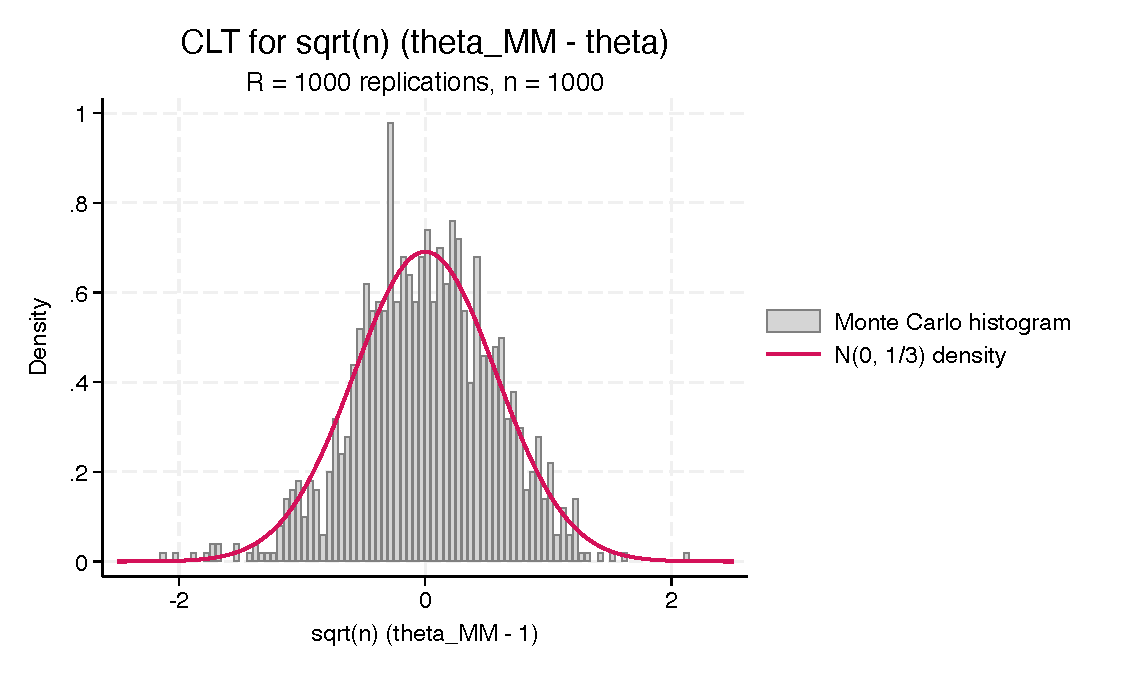
\includegraphics[width=\textwidth]{exercise1/ex1_mm_clt.pdf}
\caption{Histogram of $a_r = \sqrt n (\widehat\theta_{MM} - \theta)$ over $R = 1000$ replications, with the $\mathcal{N}(0, 1/3)$ density overlaid.}
\end{subfigure}
\hfill
\begin{subfigure}[b]{0.48\textwidth}
\centering
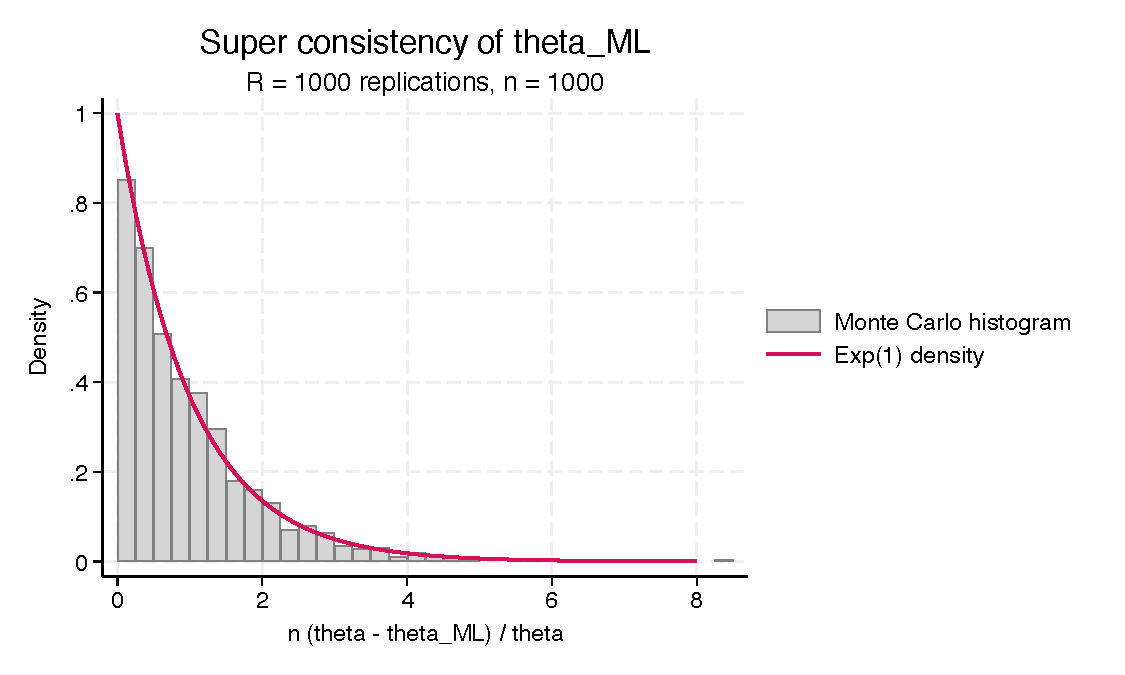
\includegraphics[width=\textwidth]{exercise1/ex1_ml_exp.pdf}
\caption{Histogram of $b_r = n(\theta - \widehat\theta_{ML})/\theta$ over $R = 1000$ replications, with the $\mathrm{Exp}(1)$ density overlaid.}
\end{subfigure}
\caption{Monte Carlo evidence for the rate gap. The left panel concentrates symmetrically around zero with spread $\sqrt{1/3}$, in line with the central limit theorem. The right panel concentrates near zero with an exponential tail of unit scale, in line with part (f).}
\label{fig:ex1_mc}
\end{figure}

The simulation confirms the analytical comparison. The MM estimator scatters around $\theta$ at scale $\theta/\sqrt{3 n}$. The ML estimator approaches $\theta$ from below at scale $\theta/n$. The visible concentration gap between the two panels of Figure~\ref{fig:ex1_mc} is the rate gap between the two limit laws.

\subsection*{Part (i)}

We now use the limit law from part (f), together with Slutsky's lemma, to build a confidence interval for $\theta$ with asymptotic coverage $1 - \alpha$.

Let $t_q = -\ln(1 - q)$ be the $q$ quantile of $\mathrm{Exp}(1)$, so that for instance $t_{0.95} = -\ln(0.05) \approx 2.996$. The proposed interval is
\[
IC(\alpha) = \left[\widehat\theta_{ML},\; \widehat\theta_{ML}\left(1 + \frac{t_{1-\alpha}}{n}\right)\right].
\]
We need to show that $P(\theta \in IC(\alpha)) \to 1 - \alpha$.

The lower endpoint takes care of itself. Since $\widehat\theta_{ML} \le \theta$ almost surely (the sample maximum is at most $\theta$), the condition $\theta \ge \widehat\theta_{ML}$ holds with probability one for every $n$. The whole question reduces to the upper endpoint, which is $\theta \le \widehat\theta_{ML}(1 + t_{1-\alpha}/n)$. Rearranging step by step,
\begin{align*}
\theta &\le \widehat\theta_{ML}\left(1 + \frac{t_{1-\alpha}}{n}\right) \\
\theta &\le \widehat\theta_{ML} + \widehat\theta_{ML} \cdot \frac{t_{1-\alpha}}{n} && \text{(distribute)} \\
\theta - \widehat\theta_{ML} &\le \widehat\theta_{ML} \cdot \frac{t_{1-\alpha}}{n} && \text{(subtract $\widehat\theta_{ML}$)} \\
\frac{n(\theta - \widehat\theta_{ML})}{\widehat\theta_{ML}} &\le t_{1-\alpha} && \text{(multiply both sides by $n/\widehat\theta_{ML} > 0$)}.
\end{align*}
Defining $W_n = n(\theta - \widehat\theta_{ML})/\widehat\theta_{ML}$, the coverage condition becomes
\[
\theta \in IC(\alpha) \;\iff\; W_n \le t_{1-\alpha},
\]
and therefore $P(\theta \in IC(\alpha)) = P(W_n \le t_{1-\alpha})$. The remaining task is the limit law of $W_n$.

Write $W_n = Z_n \cdot (\theta / \widehat\theta_{ML})$, where $Z_n = n(\theta - \widehat\theta_{ML})/\theta$ is the pivotal quantity from part (f). The first factor satisfies $Z_n \overset{d}{\longrightarrow} \mathrm{Exp}(1)$ by part (f). The second factor satisfies $\theta / \widehat\theta_{ML} \overset{P}{\longrightarrow} 1$, since $\widehat\theta_{ML} \overset{P}{\longrightarrow} \theta$ (this fact is granted in the problem and also follows from the $n$ consistency proved in part (f)) and the continuous mapping theorem applied to the map $x \mapsto \theta/x$. Slutsky's lemma in product form, namely that the product of a convergent in distribution sequence and a convergent in probability constant equals the scaled limit, then gives
\[
W_n = Z_n \cdot \frac{\theta}{\widehat\theta_{ML}} \;\overset{d}{\longrightarrow}\; \mathrm{Exp}(1) \cdot 1 = \mathrm{Exp}(1).
\]
The point $t_{1-\alpha}$ is a continuity point of the $\mathrm{Exp}(1)$ cdf, so
\[
P(\theta \in IC(\alpha)) = P(W_n \le t_{1-\alpha}) \;\longrightarrow\; P\bigl(\mathrm{Exp}(1) \le t_{1-\alpha}\bigr) = 1 - \alpha,
\]
where the last equality holds by definition of the quantile. This is the required asymptotic coverage. \qed

For $\alpha = 0.05$, $t_{0.95} = -\ln(0.05) \approx 2.996$, and the 95\% interval is
\[
IC(0.05) = \left[\widehat\theta_{ML},\; \widehat\theta_{ML}\left(1 + \frac{2.996}{n}\right)\right].
\]
At $n = 1000$ the interval has width about $0.003\, \widehat\theta_{ML}$. A standard $\sqrt n$ consistent estimator of $\theta$ would yield a confidence interval of width of order $1/\sqrt n \approx 0.03$, ten times wider. The narrow width is the practical payoff of super consistency.

\subsection*{Remark}

The problem closes with a wartime application of $\widehat\theta_{ML}$ to estimate German tank production from salvaged serial numbers. The setup differs only in that the $Y_i$ follow a discrete uniform on $\{1, \dots, \theta\}$ rather than a continuous one; the analogous results carry over with the obvious adjustments. The Allied statistical estimate of 255 tanks per month closely matched the post war recorded figure of 256, against the much higher 1400 produced by conventional intelligence. The same principle now applies in industrial intelligence and serial number analysis whenever items are issued sequentially.


\newpage

\section*{Exercise 3}
% Exercise 3, Burgess et al. (2015) replication with did_multiplegt_dyn.


\noindent \textbf{Given.} A district year panel of all 41 Kenyan districts from 1963 to 2011 (2009 district year observations, balanced). The outcome \texttt{exp\_dens\_share} is the share of national road expenditure received by a district, divided by the district's 1962 population share. The treatment \texttt{president} is a binary indicator equal to one when the district is coethnic with the serving president. The covariates \texttt{pop1962}, \texttt{area}, \texttt{urbrate1962}, \texttt{earnings}, \texttt{wage\_employment}, \texttt{value\_cashcrops} are time invariant 1963 era characteristics.\\

\noindent We are asked to use \texttt{did\_multiplegt\_dyn} to estimate dynamic treatment effects of being coethnic with the serving president on road expenditure. Justify option choices, interpret the event study. Check robustness with Burgess covariates. Investigate whether the same package can estimate the effects of switching out of coethnicity using the method in Web Appendix 1.6 of \citet{dCDH2024}.\\

 \noindent Three presidents serve over the panel: Kenyatta (Kikuyu, 1963 to 1978), Moi (Kalenjin, 1979 to 2002) and Kibaki (Kikuyu, 2003 to 2011). The treatment indicator therefore takes three regime values across 49 calendar years. Reading the data,
\begin{itemize}\setlength\itemsep{0pt}
  \item 28 districts are never coethnic with any president (controls throughout).
  \item 7 districts are coethnic under Kenyatta and Kibaki but not under Moi.
  \item 6 districts are coethnic under Moi but not under Kenyatta or Kibaki.
\end{itemize}
All 13 switching districts therefore experience their first treatment change in 1979 and their second in 2003. There is no variation in first switch dates across the switching subsample. This matters for Part 3 below.\\

\noindent All analysis is run in R. The static two way fixed effects regression is fit with \texttt{fixest}; the dynamic difference in differences estimator is the \texttt{did\_multiplegt\_dyn} function from the \texttt{DIDmultiplegtDYN} package. The full pipeline is in \texttt{analysis.R}.

\paragraph{Sanity check via static TWFE.} Before running \texttt{did\_multiplegt\_dyn} we replicate the static specification of Burgess Table 1 with a two way fixed effects regression. With district and year fixed effects and standard errors clustered by district,
\[
\widehat\beta_{\text{Col 1}} = 0.9746 \; (0.3546), \qquad \widehat\beta_{\text{Col 3}} = 0.9568 \; (0.3464),
\]
where Col 3 adds the six 1963 covariates (demography and economic activity) interacted with a linear time trend. Both numbers match Burgess Table 1 Panel A to two decimals: their Column 1 reports $0.97$ $(0.36)$ and their Column 3 reports $0.96$ $(0.35)$. Column 4 of Burgess Table 1 additionally includes economic geography indicators (corridor, border, distance to Nairobi) that are not in the supplied dataset, so we cannot replicate that column. The sample mean of \texttt{exp\_dens\_share} is $1.25$, so a coefficient near $0.97$ amounts to nearly doubling the average. This is the order of magnitude headline result of \citet{burgess2015}.

\subsection*{Part 1}

\paragraph{Option choices.}
\begin{itemize}\setlength\itemsep{0pt}
  \item \texttt{effects(5)}: report five post switch horizons. The shorter regime, Kibaki 2003 to 2011, has nine years of post switch data; five comfortably fits inside both regimes.
  \item \texttt{placebo(3)}: three pre switch periods, used to test parallel trends and no anticipation.
  \item \texttt{cluster(distnum)}: cluster standard errors at the district level. There are 41 clusters, which is at the lower end of the asymptotic comfort zone but standard for this literature.
  \item No \texttt{trends\_lin} or \texttt{controls} in this baseline. We will add the Burgess controls in Part 2.
\end{itemize}

\paragraph{Estimates.}
\begin{center}
\begin{tabular}{rrrr}
\toprule
Horizon $\ell$ & $\widehat{\mathrm{DID}}_\ell$ & SE & N switchers \\
\midrule
1 & $3.175$ & $2.181$ & 6 \\
2 & $2.853$ & $1.648$ & 6 \\
3 & $2.423$ & $1.395$ & 6 \\
4 & $3.881$ & $1.009$ & 6 \\
5 & $2.739$ & $0.469$ & 6 \\
\midrule
Av\_tot\_effect & $3.014$ & $1.171$ & 30 switch periods \\
\bottomrule
\end{tabular}
\end{center}
The joint test that all five dynamic effects are zero rejects with $p < 0.001$. Average cumulative effect over 30 switch periods is $3.01$ with SE $1.17$, significant at the 5\% level. Placebos at horizons $-1, -2, -3$ are $0.25, 0.04, 0.59$ respectively, each individually insignificant, but the joint placebo test gives $p = 0.045$ which is borderline. The latter is a mild flag against strict parallel trends.\\

 The dynamic effects are all positive and in the same order of magnitude as the static estimate, scaled up because $\mathrm{DID}_\ell$ is the long difference effect over $\ell$ periods rather than a per period effect. The largest point estimate is at $\ell = 4$ and the smallest at $\ell = 3$; the pattern is roughly flat with a peak in the middle, suggesting that the coethnicity premium materialises quickly after a regime change and persists. The event study figure shows the same pattern visually.

\begin{figure}[h]
\centering
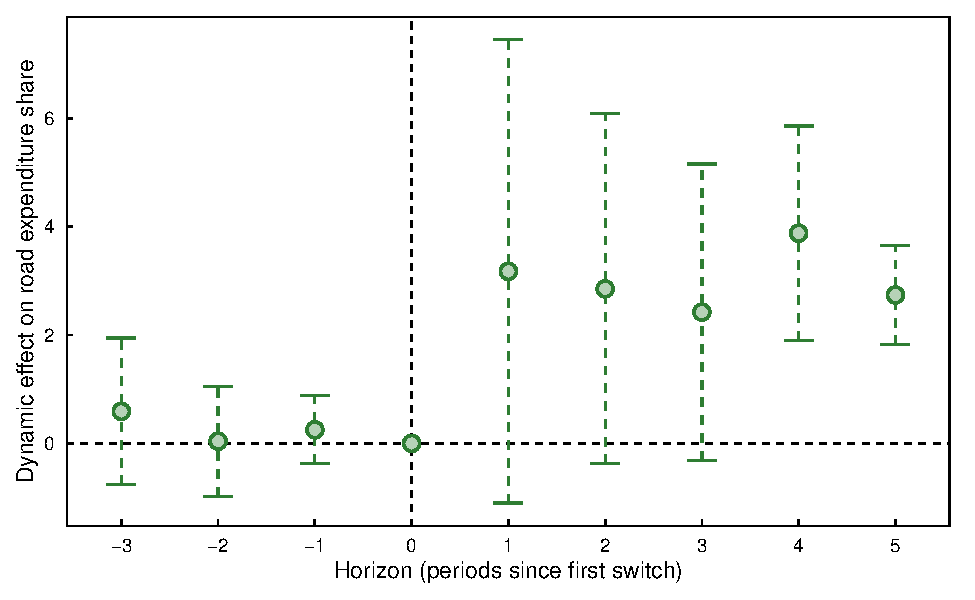
\includegraphics[width=0.75\textwidth]{exercise3/output/ex3_part1_event.pdf}
\caption{Dynamic effects of coethnicity on road expenditure, baseline specification. Horizon zero corresponds to the year of the first switch. Vertical lines are 95 percent confidence intervals based on district level clustered standard errors.}
\label{fig:ex3_part1}
\end{figure}

\subsection*{Part 2}

 The Burgess equation is
\[
\text{road}_{dt} = \gamma_d + \alpha_t + \beta \cdot (\text{coethnic district}_{dt}) + \theta \cdot \bigl(X_{d, 1963} \times (t - 1963)\bigr) + u_{dt}.
\]
Here $X_{d, 1963}$ is a vector of 1963 era district characteristics and $(t - 1963)$ is a calendar year trend. The interaction $X_{d, 1963} \times (t - 1963)$ is constant per district and linear in time, so it is a valid time varying continuous covariate from the perspective of \texttt{did\_multiplegt\_dyn}. Concretely, we construct
\[
\text{var\_tr}_{dt} = \text{var}_{d, 1963} \cdot (t - 1963)
\]
for each of the six covariates and pass them to the \texttt{controls()} option. The Burgess Table 1 sequence Cols 2 to 4 adds demographics first, then economic activity. We do this in two specifications.

\paragraph{Estimates.}
\begin{center}
\begin{tabular}{rrrrrrr}
\toprule
& \multicolumn{2}{c}{Baseline (Part 1)} & \multicolumn{2}{c}{Plus demographics} & \multicolumn{2}{c}{Plus all six} \\
\cmidrule(lr){2-3}\cmidrule(lr){4-5}\cmidrule(lr){6-7}
Horizon $\ell$ & $\widehat{\mathrm{DID}}_\ell$ & SE & $\widehat{\mathrm{DID}}_\ell$ & SE & $\widehat{\mathrm{DID}}_\ell$ & SE \\
\midrule
1 & $3.175$ & $2.181$ & $3.180$ & $2.176$ & $3.181$ & $2.177$ \\
2 & $2.853$ & $1.648$ & $2.863$ & $1.640$ & $2.865$ & $1.640$ \\
3 & $2.423$ & $1.395$ & $2.439$ & $1.380$ & $2.441$ & $1.382$ \\
4 & $3.881$ & $1.009$ & $3.902$ & $0.997$ & $3.905$ & $0.996$ \\
5 & $2.739$ & $0.469$ & $2.765$ & $0.465$ & $2.769$ & $0.463$ \\
\midrule
Av\_tot\_effect & $3.014$ & $1.171$ & $3.030$ & $1.157$ & $3.032$ & $1.158$ \\
\bottomrule
\end{tabular}
\end{center}

Adding Burgess covariates leaves point estimates essentially unchanged. Average cumulative effects move from $3.014$ to $3.030$ to $3.032$ across the three columns. Standard errors fall slightly with each additional control. The joint null on dynamic effects is rejected with $p < 0.001$ in all three specifications. The joint placebo $p$ values are $0.045$, $0.048$ and $0.049$ respectively, all borderline rather than firmly rejected.\\

The Burgess covariates therefore can be implemented in \texttt{did\_multiplegt\_dyn}, with one important caveat about interpretation. The \texttt{controls()} option accepts time varying continuous covariates and uses them to relax the parallel trends assumption: it allows the outcome trend to depend linearly on the controls. The Burgess $X_{d, 1963} \times (t - 1963)$ interactions are time varying continuous (constant per district, linear in time), so they qualify mechanically and the package runs without complaint. The interpretation is not identical to Burgess's static two way fixed effects with controls. The \citet{dCDH2024} estimator targets dynamic average treatment effects on switchers, while Burgess targets a static average effect on the treated. But the robustness exercise is in the same spirit and gives the same substantive conclusion: the dynamic estimates do not move when 1963 demographics or economic activity, interacted with the linear trend, are added. Two further notes worth keeping in mind. First, the package will not accept dummy variables in \texttt{controls()}; categorical controls have to go through the \texttt{trends\_nonparam} option instead. Our covariates are all continuous, so this limitation does not bind here. Second, with only six controls and 41 districts the asymptotic theory is being pushed.

\subsection*{Part 3}

 Web Appendix 1.6 of \citet{dCDH2024} works inside a restricted treatment structure called Design 2: $D_{g,t} = \mathbf{1}\{E_g \ge t \ge F_g\}$, where $F_g$ is the period a unit first switches into treatment and $E_g$ is the period it switches out (with $E_g = T + 1$ for units that never leave). Within Design 2 the paper defines two separately identifiable parameters, a switch in effect $\delta^+_\ell$ and a switch out effect $\delta^-_\ell$, the latter being what Question 3 asks about. The appendix's recipe for $\delta^-_\ell$ is to run \texttt{did\_multiplegt\_dyn} on the subsample of $(g, t)$ where group $g$ has already switched into treatment at or before $t$, with the treatment redefined as a $1 \to 0$ indicator and with $F_g$ included in \texttt{trends\_nonparam}. Assumption 16 of the appendix underlies the procedure: the controls must share the same switch in date $F_g$ as the unit whose switch out is being estimated.\\

The 41 Kenyan districts fall into three regime classes. Each column under a president's name shows the value of \texttt{president} during that regime.
\begin{center}
\resizebox{\textwidth}{!}{%
\begin{tabular}{lccccl}
\toprule
 & & Kenyatta & Moi & Kibaki & \\
Class & $n$ & 1963 to 78 & 1979 to 2002 & 2003 to 11 & Design 2 compatible? \\
\midrule
Never coethnic               & 28 & 0 & 0 & 0 & n.a., no switch in date \\
Moi coethnic                 & 6  & 0 & 1 & 0 & yes, $F_g = 1979,\, E_g = 2003$ \\
Kenyatta and Kibaki coethnic & 7  & 1 & 0 & 1 & no, path is not monotone \\
\bottomrule
\end{tabular}%
}
\end{center}

This mapping produces two distinct failure modes for the appendix's procedure. First, the 7 Kikuyu districts do not fit the Design 2 template at all. Design 2 requires a single contiguous block of treatment, $0 \to 1 \to 0$. The Kikuyu districts experience $1 \to 0 \to 1$ across the panel, which is not monotone and falls outside the framework in which $\delta^-_\ell$ is defined.

Second, the 6 Moi districts do fit Design 2, but the procedure still cannot be executed on them. Their switch in date $F_g$ is uniformly 1979 and their switch out date $E_g$ is uniformly 2003. Assumption 16 requires controls with the same $F_g = 1979$ that have not yet switched out by $E_g + \ell$. There are no such controls in the panel, because every Moi coethnic district switches out simultaneously in 2003 and the 7 other Moi era switchers fall outside Design 2.\\

What \texttt{analysis.R} actually runs is a coarse proxy for the appendix recipe: two \texttt{tryCatch} blocks against the package. Route A passes \texttt{switchers = "out"} on the \texttt{president} treatment. Route B recodes $\widetilde D_{dt} = 1 - D_{dt}$ and passes \texttt{switchers = "in"}. Each call is wrapped in \texttt{tryCatch()} so the script runs to completion, and the captured message is printed via \texttt{writeLines()}. Both routes return the same hard error from the R implementation, reproduced verbatim:
\begin{quote}\small\itshape
No treatment effect can be estimated. \\
\hspace*{1em}This is because Design Restriction 1 in de Chaisemartin \& D'Haultfoeuille (2024) is not satisfied in the data, given the options requested. \\
\hspace*{1em}This may be due to the fact that groups' period-one treatment is continuous, or takes a large number of values, and you have not specified the continuous option. \\
\hspace*{1em}If so, you can try to specify this option. \\
\hspace*{1em}If the issue persists even with this option, this means that all groups experience their first treatment change at the same date. \\
\hspace*{1em}In this situation, estimators of de Chaisemartin \& D'Haultfoeuille (2024) cannot be used.
\end{quote}
The error lists two possible causes. The first, a continuous or high cardinality period one treatment, does not apply because \texttt{president} is binary. The second is the one that does apply: every switching district has its first treatment change in 1979, so Design Restriction 1's staggered timing requirement is violated. The same simultaneity breaks Assumption 16 for the full appendix recipe.\\

The conclusion is that the effects of switching out of coethnicity cannot be estimated with \texttt{did\_multiplegt\_dyn} on this dataset. The obstacle is structural: the 7 Kikuyu districts fall outside Design 2 because of their not monotone treatment path, and the 6 Kalenjin districts share $F_g$ and $E_g$ so Assumption 16 has no admissible controls. The procedure in Web Appendix 1.6 would apply if Kenya had had more presidents, or if the coethnic transitions had been staggered across districts.


\newpage

\section*{Exercise 6}
% Exercise 6, four user questions to chaisemartinPackages.


\noindent \textbf{Given.} Four anonymized emails sent by \texttt{did\_multiplegt\_dyn} users to the \texttt{chaisemartinPackages} support inbox.\\

\noindent We are asked to answer each user, either by pointing them to the right resource or by explaining how to use the command correctly.\\

\noindent We reply to each user in turn. Option names and behaviour are as documented in the help file shipped with the R and Stata implementations of \texttt{did\_multiplegt\_dyn}. Where the same option is named differently in the two languages we note both.

\subsection*{Question 1}

 The student has four binary treatment variables, one per Levelling Up funding round (\texttt{pot1} switching on in 2021, \texttt{pot2} in 2022, \texttt{pot3} in 2023, \texttt{pot4} in 2024). They want the dynamic effect of each pot separately. The implicit complication, which they do not flag but matters for the answer, is that a single local authority can win more than one round, so the four treatments overlap on the same unit and the same time.\\

 \texttt{did\_multiplegt\_dyn} takes one treatment variable per call. To recover the four separate effects, run the command four times, once per pot. The package FAQ flags this design as supported, citing Web Appendix Section 3.2 of \citet{dCDH2023}, provided each treatment is binary and staggered; the pots satisfy that condition by construction. The implementation in that appendix (Theorem 6) is not to add the other pots inside \texttt{controls()}, but to restrict the sample so that the other pots are in a known state and to use \texttt{trends\_nonparam} on the cohort indicator when relevant. We follow that recipe below. The number of estimable horizons for each pot is set by the years of post switch data available before the next pot arrives.\\

 First, tabulate the pots against each other to find out whether authorities overlap. If pots are mutually exclusive across authorities (each authority wins at most one round), four independent calls without any sample restriction give four clean ATEs. If pots overlap, run four calls with the sample restrictions below: each call drops the periods where a not yet considered pot has switched on, and includes the cohort of any already considered pot in \texttt{trends\_nonparam}.\\

\begin{lstlisting}
* Stata, did_multiplegt_dyn version on SSC, current as of 2026

* Assumes a balanced authority by year panel from 2019 to 2024
* with binary indicators pot1, pot2, pot3, pot4 turning on at the funding year

* Step 0, check whether pots are mutually exclusive
tab pot1 pot2
tab pot1 pot3
tab pot2 pot3

* Step 1, Pot 1, drop authority years after later pots have arrived
preserve
keep if pot2 == 0 & pot3 == 0 & pot4 == 0
did_multiplegt_dyn outcome authority year pot1, ///
    effects(3) placebo(2) cluster(authority)
restore

* Step 2, Pot 2, restrict to cells where pot3 and pot4 are still off,
* and include the cohort of pot1 adoption in trends_nonparam
preserve
keep if pot3 == 0 & pot4 == 0
bysort authority (year): egen F_pot1 = min(cond(pot1 == 1, year, .))
replace F_pot1 = 9999 if missing(F_pot1)
did_multiplegt_dyn outcome authority year pot2, ///
    effects(2) placebo(2) cluster(authority) ///
    trends_nonparam(F_pot1)
restore

* Step 3, Pot 3, restrict to cells where pot4 is still off,
* and include the cohorts of pot1 and pot2 in trends_nonparam
preserve
keep if pot4 == 0
bysort authority (year): egen F_pot1 = min(cond(pot1 == 1, year, .))
bysort authority (year): egen F_pot2 = min(cond(pot2 == 1, year, .))
replace F_pot1 = 9999 if missing(F_pot1)
replace F_pot2 = 9999 if missing(F_pot2)
egen F_prior = group(F_pot1 F_pot2)
did_multiplegt_dyn outcome authority year pot3, ///
    effects(1) placebo(2) cluster(authority) ///
    trends_nonparam(F_prior)
restore

* Step 4, Pot 4, only the switch year is observed in 2024
* Dynamic effects cannot be estimated; report the contemporaneous effect only
bysort authority (year): egen F_pot1 = min(cond(pot1 == 1, year, .))
bysort authority (year): egen F_pot2 = min(cond(pot2 == 1, year, .))
bysort authority (year): egen F_pot3 = min(cond(pot3 == 1, year, .))
replace F_pot1 = 9999 if missing(F_pot1)
replace F_pot2 = 9999 if missing(F_pot2)
replace F_pot3 = 9999 if missing(F_pot3)
egen F_prior = group(F_pot1 F_pot2 F_pot3)
did_multiplegt_dyn outcome authority year pot4, ///
    effects(1) placebo(2) cluster(authority) ///
    trends_nonparam(F_prior)
\end{lstlisting}

 Three points to flag to the student. First, the sample restrictions are the formal mechanism in Theorem 6 of the cited Web Appendix; they cost statistical power but deliver a clean causal estimand. Second, the four pots together produce a treatment vector $(pot1_{i,t}, pot2_{i,t}, pot3_{i,t}, pot4_{i,t})$ that takes up to $2^4 = 16$ values across the panel. With a typical Levelling Up sample of roughly 300 local authorities, the cell sizes inside each subsample will be small, so dynamic effects at long horizons will be imprecise. The student should report cell counts alongside each effect, via the \texttt{save\_results} option (Question 2 below). Third, the \texttt{controls()} option is intended for time varying continuous covariates and is not the right tool for a binary staggered other treatment; passing such a treatment to \texttt{controls()} runs without error but residualises only on first differences and therefore does not capture the persistent effect of the other treatment.

\subsection*{Question 2}

 A PhD student wants the number of observations used to construct the event study graph, for the bottom of a slide.\\

 The cleanest way is the \texttt{save\_results} option, which writes a separate dataset listing each estimated effect (and each placebo) alongside its standard error, 95\% confidence interval, and the number of observations used at that horizon. After running with the option, open the saved dataset to read the per horizon counts off directly. As a complement, \texttt{ereturn list} after the command displays all stored scalars and matrices, including the total switcher count behind the average effect and the per horizon counts.\\

\begin{lstlisting}
* Stata

did_multiplegt_dyn outcome group time treatment, ///
    effects(5) placebo(3) cluster(group) ///
    save_results("ev_study_results.dta")

* Inspect the saved file
preserve
use "ev_study_results.dta", clear
list, abbreviate(20)
restore

* Alternative, query e() macros directly
ereturn list
disp "Total switcher periods behind the average: " e(N_avg_total_effect)
\end{lstlisting}

 The number reported is the count of group by period cells used in the estimation at each horizon, which is the natural quantity to put on a slide. It is not the count of distinct switching units, which is typically smaller (one unit contributes multiple cells across horizons). If the student prefers the number of distinct switchers behind the graph, they should construct it from the panel itself (number of unique \texttt{group} values where \texttt{treatment} changes), not from the package output.

\subsection*{Question 3}

 An R user has a product by month panel with 60 monthly observations per product. They are running \texttt{did\_multiplegt\_dyn} with \texttt{time = "linear\_month"} (a $1$ to $60$ index) and want to control for monthly seasonality, motivated by recurring discount seasons.\\

 The command already controls for any aggregate price shock that hits every product in the same month, because it includes a time fixed effect at the level of the time variable. With \texttt{time = "linear\_month"} taking values $1, 2, \dots, 60$, each calendar month in the panel has its own fixed effect, so the cross product seasonal pattern (the heavy December discount, the August lull) is absorbed automatically. The user does not need to add anything for the seasonality they describe.\\

The reason \texttt{controls} cannot take month dummies is mechanical: the option residualises the first difference of the outcome on the first differences of the controls, so a dummy contributes only at its turn on date, not at the level. For seasonal controls that vary across product categories rather than across products, the right tool is \texttt{trends\_nonparam}, which interacts the time fixed effects with a time invariant group level variable. The most common application is a product category indicator that allows electronics, apparel and food to follow distinct calendar trends.

\begin{lstlisting}
# R, current did_multiplegt_dyn signature

# Time fixed effects absorb aggregate seasonality automatically
mod_base <- did_multiplegt_dyn(
  final_sample, "log_price", "prod_ID", "linear_month", "new_treatment",
  effects = 12, placebo = 12, cluster = "prod_ID"
)

# If different product categories experience different seasonality,
# create a time invariant category indicator at the product level
# and pass it to trends_nonparam
mod_cat <- did_multiplegt_dyn(
  final_sample, "log_price", "prod_ID", "linear_month", "new_treatment",
  effects = 12, placebo = 12, cluster = "prod_ID",
  trends_nonparam = "category"
)
\end{lstlisting}

 \texttt{trends\_nonparam} requires the variable to be time invariant at the group level: each \texttt{prod\_ID} must have one constant category. If category itself varies over time for a given product (e.g.\ reclassifications), the option will not accept it and the user must either pick a coarser, stable grouping or drop the time varying category.

\subsection*{Question 4}

 A PhD student wants to estimate the dynamic effect of a main treatment while accounting for a second policy that hits treated groups later, at staggered horizons. They want to add this second policy as an extra fixed effect inside \texttt{did\_multiplegt\_dyn}.\\

 The command does not accept extra fixed effects beyond group and time. For a binary staggered second policy that contaminates the post treatment horizons of the focal estimator, Theorem 6 of \citet{dCDH2023}, Web Appendix Section 3.2, prescribes a sample restriction, not a control variable. The cleanest implementation here is to drop the (group, time) cells where the second policy has already arrived, then run \texttt{did\_multiplegt\_dyn} on the focal treatment in that restricted panel. The estimator then targets the dynamic effect of the main treatment uncontaminated by the second policy, at the cost of any horizon where the second policy has begun to contaminate the data.\\

If horizons longer than the second policy's typical arrival lag are still of interest, a complementary strategy from page 49 of the same Web Appendix is to include the cohort indicator of the second policy in \texttt{trends\_nonparam}, which allows counterfactual trends to differ by the timing of contamination. The two approaches answer slightly different questions: the sample restriction estimates the effect in the regime where the second policy has not yet arrived; the \texttt{trends\_nonparam} approach uses the full panel but assumes parallel trends within each second policy cohort.\\


\begin{lstlisting}
* Stata

* Main treatment T_main (binary, staggered), second policy T_second (binary, staggered)

* Approach 1, primary: restrict the sample to cells before the second policy arrives
preserve
keep if T_second == 0
did_multiplegt_dyn outcome group time T_main, ///
    effects(5) placebo(3) cluster(group)
restore

* Approach 2, complementary: keep the full sample, but allow trends to differ
* by the cohort of second policy adoption (F_T2 = first period of T_second == 1)
bysort group (time): egen F_T2 = min(cond(T_second == 1, time, .))
replace F_T2 = 9999 if missing(F_T2)
did_multiplegt_dyn outcome group time T_main, ///
    effects(5) placebo(3) cluster(group) ///
    trends_nonparam(F_T2)
\end{lstlisting}

 Two limits worth flagging. First, the procedures above cover binary staggered second treatments. If the second policy varies in intensity or unwinds and switches back on, the user is outside the regime in which Theorem 6 was proved, and they should consult \citet{dCDH2023} directly to assess whether their case fits. Second, the dynamic multi treatment problem is still active research. The static identification result in \citet{dCDH2023} is the cleanest theoretical anchor; the sample restriction and \texttt{trends\_nonparam} recipes above are the dynamic adaptations the package supports, and the staggered binary assumption is the empirical price for them.


\newpage

\section*{Exercise 7}
% Exercise 7, GitHub change review.

\noindent \textbf{Given.} A GitHub commit dated 24 July 2024 in \texttt{Credible-Answers/did\_multiplegt\_dyn}, the team's current public repository for the package.\\

\noindent We are asked to summarise the purpose of the change, identify the initial issue it addresses where relevant, and explain any new econometric tools with formulas.\\

\noindent The date in fact carries two commits seconds apart. The first, \texttt{b72fe45}, archives the prior version of the \texttt{.ado} and \texttt{.sthlp} files as the SSC submission snapshot for that date. The second, \texttt{b3849a3}, is the substantive code change. The discussion below targets \texttt{b3849a3}; \texttt{b72fe45} is treated as a release housekeeping commit.

The substantive commit adds one new econometric tool (a Wald test of joint nullity of all dynamic effects), fixes one bug reported by a user (issue 72), and bundles three smaller user experience improvements. We treat each in turn.

\subsection*{New econometric tool, joint Wald test that all dynamic effects are zero}

 \texttt{did\_multiplegt\_dyn} already shipped two diagnostics: an F test of joint nullity for the placebos (assess parallel trends) and, under the \texttt{effects\_equal} option, an F test that all dynamic effects are equal to one another (assess flatness of the event study). What was missing was the dual to the placebo test on the post side, namely a single test of the strict null that the treatment has no dynamic effect at any horizon. The commit adds that test and prints it automatically whenever at least two effects are requested and all of them are estimable.\\

 Let $L$ be the number of post horizons requested (the scalar \texttt{l\_XX} in the code), let $\widehat{\mathrm{DID}}_\ell$ denote the estimated effect at horizon $\ell$ (the macro \texttt{DID\_l\_XX}), and stack the effects into the column vector
\[
\widehat{\boldsymbol{\beta}} = \bigl(\widehat{\mathrm{DID}}_1, \widehat{\mathrm{DID}}_2, \dots, \widehat{\mathrm{DID}}_L\bigr)^{\prime} \in \mathbb{R}^{L}.
\]
The code builds the estimated covariance matrix $\widehat{\boldsymbol{\Sigma}} \in \mathbb{R}^{L \times L}$ entry by entry. The diagonal entries are the squared standard errors already stored from the main estimation,
\[
\widehat{\boldsymbol{\Sigma}}[\ell, \ell] = \widehat{\mathrm{se}}_\ell^{\,2}.
\]
The off diagonal entries use the identity
\[
\mathrm{Var}(U_\ell + U_j) = \mathrm{Var}(U_\ell) + \mathrm{Var}(U_j) + 2\, \mathrm{Cov}(U_\ell, U_j),
\]
where $U_\ell$ is the unit level influence function contribution to the horizon $\ell$ effect (stored across observations as \texttt{U\_Gg\_var\_glob\_l\_XX}). Solving for the covariance,
\[
\widehat{\mathrm{Cov}}(U_\ell, U_j) = \tfrac{1}{2}\bigl[\widehat{\mathrm{Var}}(U_\ell + U_j) - \widehat{\mathrm{se}}_\ell^{\,2} - \widehat{\mathrm{se}}_j^{\,2}\bigr].
\]
The code constructs $U_\ell + U_j$ at the observation level, squares it, sums across the panel and divides by $G^2$ (the squared group count) to recover $\widehat{\mathrm{Var}}(U_\ell + U_j)$; the off diagonal entry is then filled in symmetrically. The test statistic is the standard Wald form
\[
W = \widehat{\boldsymbol{\beta}}^{\,\prime}\, \widehat{\boldsymbol{\Sigma}}^{-1}\, \widehat{\boldsymbol{\beta}}.
\]
Under the null $H_0: \delta_\ell = 0$ for all $\ell \in \{1, \dots, L\}$ and the asymptotic normality result for $\widehat{\boldsymbol{\beta}}$ from \citet{dCDH2024}, Theorem 1, $W$ converges in distribution to a $\chi^2_L$ variate, and the $p$ value is computed as
\[
\widehat{p}_{\text{joint}} = 1 - F_{\chi^2_L}(W).
\]
The scalar is stored as \texttt{e(p\_jointeffects)} and printed at the bottom of the standard output table, below the dynamic effects.\\

 When the user passes the \texttt{normalized} option, the influence functions $U_\ell$ are rescaled by the corresponding cumulative incremental dose $\delta_D^\ell$ (the scalar \texttt{delta\_D\_l\_global\_XX}) before the off diagonals are computed, so the test is performed on the normalized estimator $\widehat{\mathrm{DID}}_\ell^n = \widehat{\mathrm{DID}}_\ell / \delta_D^\ell$. When the user passes the \texttt{bootstrap} option, the analytical $\widehat{\boldsymbol{\Sigma}}$ is replaced by the bootstrapped covariance matrix \texttt{bs\_var\_cov\_XX}, leaving the rest of the construction unchanged.\\

 The pre existing \texttt{effects\_equal} routine tests $H_0: \delta_1 = \delta_2 = \dots = \delta_L$, that is, flatness of the event study. The new test targets $H_0: \delta_1 = \delta_2 = \dots = \delta_L = 0$, that is, no effect at any horizon. Rejecting the new test does not imply rejecting the equality test, and vice versa: a perfectly flat but nonzero event study would pass the equality test and fail the joint nullity test. The two diagnostics are complementary and the commit retains both. A line in the code, commented \texttt{// Modif Felix: this scalar is already initalized above and would now be overwritten when it should not be}, prevents the older equality routine from re initialising the joint nullity flag that the new code sets.

\subsection*{Bug fix, issue 72: \texttt{inv\_Denom\_4\_XX not found}}

A user (Yuankun Li, Tsinghua University) reported on 20 July 2024 that running \texttt{did\_multiplegt\_dyn} with the \texttt{controls()} option on a panel of five binary policy variables produced the error
\begin{quote}\small\itshape
inv\_Denom\_4\_XX not found
\end{quote}
for one of the five treatments while the other four ran without issue. Felix Knau (member of the team) closes the issue on 25 July with the message that the latest update fixes the bug; the latest update is \texttt{b3849a3}.

The root cause is in the loop that adjusts the influence function for the controls. For each value $d$ of the period one treatment (variable \texttt{d\_sq\_int\_XX}) the code constructs a denominator matrix \texttt{inv\_Denom\_d\_XX} and inverts it; the inversion fails silently if the number of useful residual cells at that level (the scalar \texttt{useful\_res\_d\_XX}) is at most one, because the underlying regression has fewer observations than parameters. The control adjustment loop then references the missing matrix and Stata stops on the not found error. The fix adds the guard
\begin{quote}\small\ttfamily
if (scalar(useful\_res\_`l'\_XX) > 1)\{ \ldots \}
\end{quote}
around the inner sum over status quo levels, in both the effect branch (lines around 4247 in the diff) and the placebo branch (lines around 4590). Levels with at most one useful residual are skipped silently, the loop proceeds across the remaining levels, and the rest of the estimation completes. The fix is conservative in spirit: it does not invent a degenerate inverse, it simply drops the contributions that cannot be computed.

\subsection*{Three user experience improvements}

These do not change the econometrics, but they are visible to users and worth listing because each closes a specific failure mode.

\begin{enumerate}
\item \textbf{Tightened input check for \texttt{bootstrap(k)}.} The pre existing check rejected $k < 0$ as invalid. The new check rejects $k < 2$, on the rationale that a single bootstrap replication produces a degenerate variance estimate. The error message is updated correspondingly: \textit{the input of the \texttt{bootstrap()} option has to be a positive integer greater than 1}.

\item \textbf{Validation inside \texttt{predict\_het}.} If the user invokes \texttt{predict\_het} but supplies no variable (the substring before the comma in the option's argument is empty), the new code prints a warning and silently ignores the option rather than letting the downstream code fail on an empty variable list.

\item \textbf{Bootstrap loop with zero placebos.} The bootstrap routine builds a list of coefficient names to be resampled by iterating over both effect and placebo horizons. The pre existing code unconditionally called \texttt{numlist "1/`=l\_placebo\_XX'"}, which errors out when \texttt{l\_placebo\_XX} equals zero (no placebos requested). The fix wraps the placebo segment of the loop in \texttt{if `=l\_placebo\_XX'>0\{\ldots\}}, leaving the effect segment unchanged.


\end{enumerate}





\bibliographystyle{plainnat}
\bibliography{refs}

\section*{AI use}

Every numerical result in this report was reproduced from the supplied data, and every citation was verified against the published paper or working-paper PDF in the \texttt{Papers/} folder. Claude (Anthropic) served as a syntax assistant for the Stata Monte Carlo loop in Exercise 1 and as a drafting aide for the LaTeX writeup throughout. Mathematical derivations, the design of Part 3 of Exercise 3, the diagnosis of the user questions in Exercise 6, and the reading of commit \texttt{b3849a3} and issue 72 in Exercise 7 are mine; the package help file and the relevant theorems from \citet{dCDH2023} and \citet{dCDH2024} were read directly rather than summarised through the model. A clean transcript of the substantive AI exchange for Exercise 1 is included in \texttt{ai\_transcripts/}, formatted per the template I used at the top of each prompt: context, conceptual framework already in place, the narrow task, the constraints, and the verification step.

\end{document}
